\documentclass{article}

\usepackage[english]{babel}
\usepackage{amsmath}
\usepackage{amssymb}
\usepackage{amsthm}
\usepackage[font=small]{caption}
\usepackage{cite}
\usepackage{graphicx}

\newtheorem{algorithm}{Algorithm}
\newtheorem{definition}{Definition}
\newtheorem{example}{Example}
\newtheorem{lemma}{Lemma}
\newtheorem{proposition}{Proposition}
\newtheorem{remark}{Remark}

%---------------------------------------------------------------

\title{Topics to follow up on from work on seedin}
\author{
\textsc{Guillaume Filion} \\ [1ex]
\normalsize CRG, Barcelona
}
\date{\today}

%---------------------------------------------------------------
%---------------------------------------------------------------


\begin{document}

\maketitle

\begin{abstract}
The abstract will come later.
\end{abstract}


%---------------------------------------------------------------
%---------------------------------------------------------------



%%%%%%%%%%%%%%%%%% sampling seedless reads %%%%%%%%%%%%%%%%%%%%%

\section{Sampling seedless reads}

It is trivial to use the error models presented above to sample reads.
This approach is suboptimal if we are only interested in seedless
reads, because they may be sampled at a very low rate. Sampling
seedless reads at maximum rate, \textit{i.e.} without rejection is
desirable when they occur at low frequency under the given error model.
The question is how to sample the reads with a frequency that is equal to
their expected occurrence among seedless reads.

Here analytic combinatorics offers a simple way to achieve this via the
symbolic method. The combinatorial construction associated with an
error model gives us a handle for a sampling algorithm. At each iteration
of the process, we simulate the length of an error-free interval, which is
a number between $0$ and $d-1$, followed by an error. The probabilities
of these $d$ possible outcomes are computed thanks to asymptotic formulas
given by proposition§~\ref{th:ass}.




\subsection{Substitutions only}
\label{sec:smplsub}

We start from the weighted generating function of reads, namely

\begin{equation}
\tag{\ref{eq:Rsub}}
R(z) = \frac{1+F(z)}{1-pz\big( 1+F(z) \big)}.
\end{equation}

Rearranging the terms, we see that this expression is also equal to

\begin{equation}
\label{eq:altSp}
R(z) = \frac{1}{1-pz} \cdot \frac{1}{1-F(z)\frac{pz}{1-pz}} \cdot
\big(1+F(z)\big) = H(z) \cdot B(z) \cdot T(z).
\end{equation}

Expression (\ref{eq:altSp}) indicates that reads can be viewed as
combinations of three objects with respective weighted generating
functions $H(z)$, $B(z)$ and $T(z)$, referring to ``head'', ``body'' and
``tail''.

Recall from proposition~\ref{th:sequences} that if $A(z)$ is the weighted
generating function of the set $\mathcal{A}$, then $1/(1-A(z))$ is the
weighted generating function of $\mathcal{A}^*$, the set of sequences of
objects from $\mathcal{A}$. Since $pz$ is the weighted generating function
of substitutions, $H(z)$ is directly recognized as the weighted generating
function of sequences of substitutions.

Similarly, $B(z)$ appears as the weighted generating function of sequences
of objects that we will call ``S-monomers'', identified by the weighted
generating function $F(z)pz/(1-pz)$. The S-monomers themselves consist
of two objects. The term $F(z)$ is the weighted generating function of
error-free intervals, and according to proposition~\ref{th:sequences}, the
term $pz/(1-pz)$ is the weighted generating function of non-empty
sequences of substitutions. In other words, the body is a sequence of
S-monomers, each of which is an error-free interval and a sequence of at
least one substitution.

Finally, $T(z)$ is the sum of $1$, the weighted generating function of the
empty object, and $F(z)$, the weighted generating function of error-free
intervals. This means that the tail is either empty or an error-free
interval.


\begin{definition}
An \textbf{S-monomer} is an error-free interval followed by a
non-empty sequence of substitutions.
\end{definition}

\begin{figure}[h]
\centering
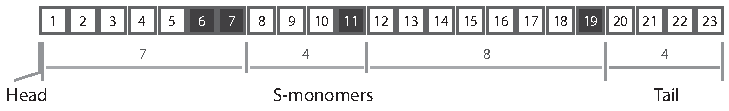
\includegraphics[scale=0.95]{sketch_S_monomers.pdf}
\caption{\textbf{S-monomers}. Reads can be segmented into a head, a
sequence of monomers and a tail. When errors are substitutions only, the
monomers are called ``S-monomers'' and they consist of an error-free
interval and a sequence of at least one substitution. In this example, a
read of size $23$ with four substitutions (black squares) is segmented in
three S-monomers and a tail (the head is empty).}
\label{fig:sketchsubint}
\end{figure}

\begin{remark}
In this section and the following two, we will use $\Delta$ as a generic
symbol to denote exponentially small terms.
\end{remark}

The key observation is that if we remove a monomer from a seedless read,
the read remains seedless. Let $(a,b)$ denote the size of a monomer with
an error-free interval of size $a$ followed by a sequence of substitutions
of size $b$. Assume that $a < d$ such that the monomer does not contain a
seed. The probability that the first monomer of a read is $(a,b)$ is
$q^ap^b$. The probability that a read with this monomer is seedless is
$C/z_1^{k+1-a-b} + \Delta$. Since the probability that a read of size $k$
contains no seed is $C/z_1^{k+1} + \Delta$, the probability that a 

To generate the read, we first sample the head, then each S-monomer, then
the tail. A seedless read of size $k$ that starts with $m$ or more
substitutions is a sequence of $m$ substitutions followed by a seedless
read of size $k-m$, which has probability $p^m \cdot (C/z_1^{k-m+1} +
\Delta)$. Since seedless reads of size $k$ occur with probability
$C/z_1^{k+1} + \Delta$, the probability that a seedless read starts with
$m$ or more substitutions is approximately $(pz_1)^m$. In short, we can
sample the head as an exponential variable with parameter $pz_1$ (we
will see below that $pz_1 < 1$).

Let $(a,b)$ denote the first monomer of a seedless read of size $k$, where
$a$ is the length of a bounded error-free interval, and $b$ is the length
of a sequence of at least one substitution. The probability of this
monomer is $q^ap^b$. Removing the monomer gives a seedless read of size
$k-a-b$, whose probability of occurrence is $C/z_1^{k+1-a-b}+\Delta$. By
the same argument as above, the probability that the first monomer is
$(a,b)$ is thus approximately equal to $(qz_1)^a(pz_1)^b$.

The marginal distributions of this variable are $(qz_1)^apz_1$ and
$F(z_1)(pz_1)^b$.

Note that $pz_1 + pz_1qz_1 + \ldots + pz_1(qz_1)^{d-1} = 1$ because by
definition, $z_1$ is a root of the polynomial $1-pz(1+F_d(z)) =
1-pz(1+qz+\ldots+pz_1(qz)^{d-1})$. This shows that the terms
$pz_1(qz_1)^{m-1}$ can be interpreted as probabilities, giving a
straightforward way to sample the first S-interval. This is a
geometric distribition with parameter $qz_1$, conditioned on the values
$0, 1, \ldots, d-1$.

The process can be repeated to produce the next S-intervals.
When the generated read has size $k$ or greater, the process is stopped,
and the nucleotides beyond $k$ are removed. The analytic combinatorics
approaches directly yields a simple and efficient scheme to sample
seedless reads. Once again, it is unclear how one may obtain the same
result with a different approach.

\begin{example}
Say that we want to sample a read of size $k=100$, without seed of size
$d=17$, with substitution rate $p = 0.1$. We start by finding $z_1$, the
dominant singularity of the weighted generating function. Referring to
example~\ref{ex:num1}, we recall that $z_1 \approx 1.0268856$.

This value at hand, we compute the terms $P(m = 1) \approx pz_1 \approx
0.10269$, $P(m = 2) \approx pz_1qz_1 \approx 0.09490$, $P(m = 3) \approx
pz_1(qz_1)^2 \approx 0.08771$ \textit{etc}. A uniform pseudo random
generator yields $P(m \leq 8) < 0.68414 < P(m \leq 9)$, so the read starts
with an error-free interval of size $8$ followed by a substitution.  The
next call to the pseudo random generator yields $0.08860 < P(m \leq 1)$,
so we append a substitution to the read, for a total size of $10$.

The process must be repeated until the total size is at least $100$. At
that point, the excedent nucleotides, if any, are removed so that the size
of the read is exactly $100$.
\end{example}




\subsection{Substitutions and deletions}

We can use the same principle to sample seedless reads under the error
model descrbibed in section~\ref{sec:deletions}.

\begin{equation}
\tag{\ref{eq:Sdel}}
S(z) = \frac{1+F_d(z)(1-\delta)}{1-pz-\big(pz(1-\delta)
  + \delta\big) F_d(z)}.
\end{equation}

Using proposition~\ref{th:sequences}, can express (\ref{eq:Sdel}) as

\begin{equation*}
  \sum_{n=0}^\infty \left(F_d(z) \left( \delta + \frac{pz}{1-pz}\right)
  \right)^n \frac{1+(1-\delta)F_d(z)}{1-pz}.
\end{equation*}

This expression shows that under the error model of substitutions and
deletions, seedless reads can be considered as sequences of monomers with
weighted generating function $F_d(z)\big( \delta + pz / (1-pz) \big)$,
followed by a terminator with weighted generating function
$(1+F_d(z)(1-\delta))/(1-pz)$.

$F_d(z)$ is the weighted generating function of error-free intervals of
size less than $d$ and the term $\delta + pz/(1-pz)$ is the weighted
generating function of a deletion or a non-empty sequences of
substitutions. This justifies the following definition.

\begin{definition}
An \textbf{SD-interval} is an error-free interval of size less than $d$,
followed by either a deletion or a non-empty sequence of substitutions.
\end{definition}

Monomers are thus an error-free interval followed by either
a deletion or a non-empty sequence of substitutions

(Figure~\ref{fig:sketchdelint}).
\begin{figure}[h]
\centering
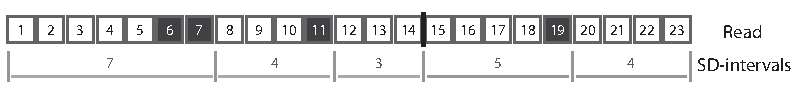
\includegraphics[scale=0.90]{sketch_SD_intervals.pdf}
\caption{\textbf{Decomposition into SD-intervals}. When
errors consist of either substitutions or deletions, we can segment reads
in SD-intervals. Example of a read of size $23$ with $4$ substitutions
(black squares) and $2$ deletions (bold vertical bars) segmented in $5$
SD-intervals.}
\label{fig:sketchdelint}
\end{figure}

The second generating function, $(1+F_d(z)(1-\delta))/(1-pz)$ consists of
two terms. The first, $1/(1-pz)$ is the same as the head of an
SD-interval. The second, $1+F_d(z)(1-\delta)$ is the weighted generating
function of either the empty object, or an error-free interval not
followed by a deletion. Such objects account for the fact that the right
end of the read may not coincide with the tail of a deletion interval. In
this case, the read may not end with a deletion (this case is covered by
the tail of SD-intervals).

We can now describe a method to sample seedless reads with this error
model. Assume that the read size $k$, the minimum seed length $d$, the
substitution rate $p$ and the deletion rate $\delta$ are given. We want to
generate a read according to its probability of occurrence among seedless
reads.

Say that a read starts with an SD-interval 
. The
probability of such a read is $p^a \cdot (1-\delta)^{b-1}q^b \cdot
\delta \cdot (C/z_1^{k+1-a-b} + \Delta)$ if the tail is a deletion, or
$p^a \cdot (1-\delta)^{b-1}q^b \cdot (1-\delta)p \cdot (C/z_1^{k+1-a-b-1}
+ \Delta)$ if the tail is a substitution. Since the occurrence of
seedless reads of size $k$ is $C/z_1^{k+1} + \Delta$, this read occurs
among seedless reads with approximate probabilities $(pz_1)^a
(1-\delta)^{b-1}(qz_1)^b \delta$ if the tail is a deletion or $(pz_1)^a
(1-\delta)^{b-1}(qz_1)^b (1-\delta)pz_1$ if the tail is a substitution.

As in section~\ref{sec:smplsub}, we sample seedless reads one SD-interval
at at time. Summing over all possible values of $a$ and $b$, and over the
two types of tail, we obtain a total probability equal to

\begin{equation*}
\sum_{a=0}^\infty \sum_{b=1}^{d-1} (pz_1)^a (1-\delta)^{b-1}(qz_1)^b
\big(\delta + (1-\delta)pz_1 \big) = \frac{F_d(z_1)(\delta +
(1-\delta)pz_1)}{1-pz_1} = 1.
\end{equation*}

The last equality comes from the fact that by definition, $z_1$ is a root
of the polynomial $1-pz-F_d(z_1)(\delta +(1-\delta)pz_1)$. Since all the
terms of the sum are positive, they define a proper probability
distribution and since the terms are independent, we can use the marginal
distributions to sample the head, the body and the tail.

According to the marginal distribution, the probability that the head has
size $a \geq 0$ is $(1-pz_1)(pz_1)^a$. Similarly, the probability that the
body has size $b$, for $1 \leq b \leq d-1$, is $(1-\delta)^{b-1}(qz_1)^b /
F_d(z_1)$, and the probability that the tail is a deletion is $\delta /
(\delta + (1-\delta)pz_1)$. With these probabilities we can sample the
head, the body and the tail of SD-intervals until size $k$ is
reached, and delete the nucleotides beyond $k$.

\begin{example}
Say that we want to sample a read of size $k=100$, without seed of size
$d=17$, with substitution rate $p = 0.05$ and deletion rate $\delta=0.15$.
We start by finding $z_1$, the dominant singularity of the weighted
generating function. Referring to example~\ref{ex:num2}, $z_1 \approx
1.006705$.

\begin{enumerate}

\item
From the term $pz_1 \approx 0.050335$, we compute $P(a=0) = 1-pz_1
\approx 0.94967$, $P(a \leq 1) = P(a=0) + (1-pz_1)pz_1 \approx 0.99747$
\textit{etc}. Using a pseudo-random number generator, we obtain $0.6671961
< P(a=0)$ a we thus set the size of the head to $0$ (\textit{i.e.} there
is no initial substitution).

\item
For the body, we compute $F_d(z_1) \approx 4.96081$, which yields
$P(b=1) = qz_1/F_d(z_1) \approx 0.19279$, $P(b \leq 2) = P(b=1)
+ (qz_1)^2(1-\delta)/Fd(z_1) \approx 0.34950$ \textit{etc}. Using a
pseudo-random number generator gives $P(b \leq 11) < 0.875563 < P(b
\leq 12)$. So we set the size of the error-free interval to $12$.

\item
To sample the tail, we compute $\Delta = \delta / (\delta +
(1-\delta)pz_1) \approx 0.77807$.  Using a pseudo-random number generator,
we obtain $0.37722 < \Delta$, so the sampled SD-interval consists of
$12$ correct nucleotides, followed by a deletion.
\end{enumerate}

The process must be repeated until the total size is at least $100$. At
that point, the excedent nucleotides are removed so that the size of the
read is exactly $100$.
\end{example}

\begin{remark}
In case the reads are generated from some template, the number of
nucleotides that are deleted in each run of deletions must be estimated
and computed separately.
\end{remark}




\subsection{Substitutions, deletions and insertions}

Finally, we can sample seedless reads under the more complex error model
of subsitutions, deletions and insertions described in
section~\ref{sec:insertions}. Recall that under this model, the weighted
generating function of seedless reads is

\begin{equation}
\tag{\ref{eq:Sindel}}
S(z) = \frac{(1-r)\big( 1-(\tilde{r}-r)z \big) \left(1+(1-\delta)F_d(z)
\right)}{1-a(z)-b(z)F_d(z)},
\end{equation}

\noindent
where $a(z)$ and $b(z)$ are second degree polynomials defined as

\begin{gather*}
a(z) = r-\big((p+\tilde{r})r-\tilde{r}-p\big)z
- p(\tilde{r}-r)z^2\text{, and} \\
b(z) = \delta(1-r) - \big((\tilde{r}\delta-(1-\delta)p)(1-r)
-(1-\tilde{r})r\big)z -(1-\delta)p(\tilde{r}-r)z^2.
\notag
\end{gather*}


Using proposition~\ref{th:sequences}, we can express (\ref{eq:Sindel}) as

\begin{equation*}
  \sum_{n=0}^\infty \left( \frac{b(z)F_d(z)}{1-a(z)}
  \right)^n \frac{(1-r)\big( 1-(\tilde{r}-r)z \big)
\left(1+(1-\delta)F_d(z)\right)}{1-a(z)}.
\end{equation*}

As in the previous cases, seedless reads appear as sequences of
combinatorial objects followed by a terminator. The monomers have
weighted generating function $b(z)F_d(z)/(1-a(z))$ and the terminators
have weighted generating function $(1-r)\big( 1-(\tilde{r}-r)z
\big)\left(1+(1-\delta)F_d(z)\right)/(1-a(z))$.

From figure~\ref{fig:insertions} and from the general framework presented
in section~\ref{sec:substitutions}, the transfer matrix of 
a sequence of substitutions and insertions is

\begin{equation*}
M(z) = \left(
\begin{matrix}
pz      & rz  \\
\frac{1-\tilde{r}}{1-r}pz & \tilde{r}z
\end{matrix}
\right).
\end{equation*}

Such a sequence can start with a substitution or a deletion, so the vector
of initial objects $U(z)$ is equal to $(pz, rz)$. The sequence can end on
a substitution with weight $1$, or on an insertion with weight
$(1-\tilde{r})/(1-r)$, so the vector of final objects $V$ is equal to $(1,
(1-\tilde{r})/(1-r))^T$.

Applying proposition~\ref{th:TM2WGF}, the weighted generating function of
non-empty sequences of substitutions and insertions is see to be equal to
$U(z) \cdot M_*(z) \cdot V$, where $M_*(z) = (I-M(z))^{-1}$. The weighted
generating function of a deletion or a sequence of substitutions and
insertions is thus equal to $\delta + U(z) \cdot M_*(z) \cdot V$. It can
be verified that this expression is equal to $b(z)/(1-a(z))$.

If a seedless read of size $k$ starts with an SDI-interval of size
$(h,m)$, it consists of a head of size $h$, an error-free interval of size
$m$, and a seedless read of size $k-(h+m)$. The probability of such a read
is $p^a \cdot \ldots \cdot (C/z_1^{k+1-h-m} + \Delta)$. Since the
probability of seedless reads of size $k$ is $C/z_1^{k+1} + \Delta$, the
occurrence of this read among seedless reads is approximately







\section{Average size of error-free intervals}
\label{sec:avsz}

Another quantity of interest is the average size of error-free intervals.
for this we need to mark two quantites: the total size of intervals and
the number of intervals. A question we need to decide straight away is
whether an interal of size zero is an interval. We will get two different
answers, depend on whether we answer yes or no to this question.

We start from expression

\begin{equation}
\tag{\ref{eq:altSp}}
(1+F_d(z)) \sum_{n=0}^\infty \big( pz(1+F_d(z)) \big)^n.
\end{equation}

We can label every error-free interval with the variable $u$ by replacing
$F_d(z)$ with $uF_d(z)$. We can also count the cumulative size of
error-free intervals through the variable $v$ by replacing $F_d(z)$ with
$F_d(zv)$. We thus obtain the weighted generating function of three
variables

\begin{equation*}
S(z,u,v) = (1+uF_d(zv)) \sum_{n=0}^\infty \big( pz(1+uF_d(zv)) \big)^n =
\frac{1+uF_d(zv)}{1-pz(1+uF_d(zv))}.
\end{equation*}

We first derive with respect to $v$ and then integrate with
respect to $u$.

\begin{equation*}
\frac{\partial S(z,u,v)}{\partial v} \Bigr|_{\substack{\\v=1}} =
 \frac{zuF'_d(z)} {\big( 1-pz(1+uF_d(z)) \big)^2}.
\end{equation*}

Now, to integrate with respect to $u$, we need to do the partial fraction
decomposition of the ratio

%\bibliography{pubmed,extra}
%\bibliographystyle{plain}

%----------------------------------------------------------------

\end{document}

%gs -dNoOutputFonts -sDEVICE=pdfwrite -o out.pdf latex.pdf 
